\section{W4-5: GRASP}
General Responsibility Assignment Software Patterns
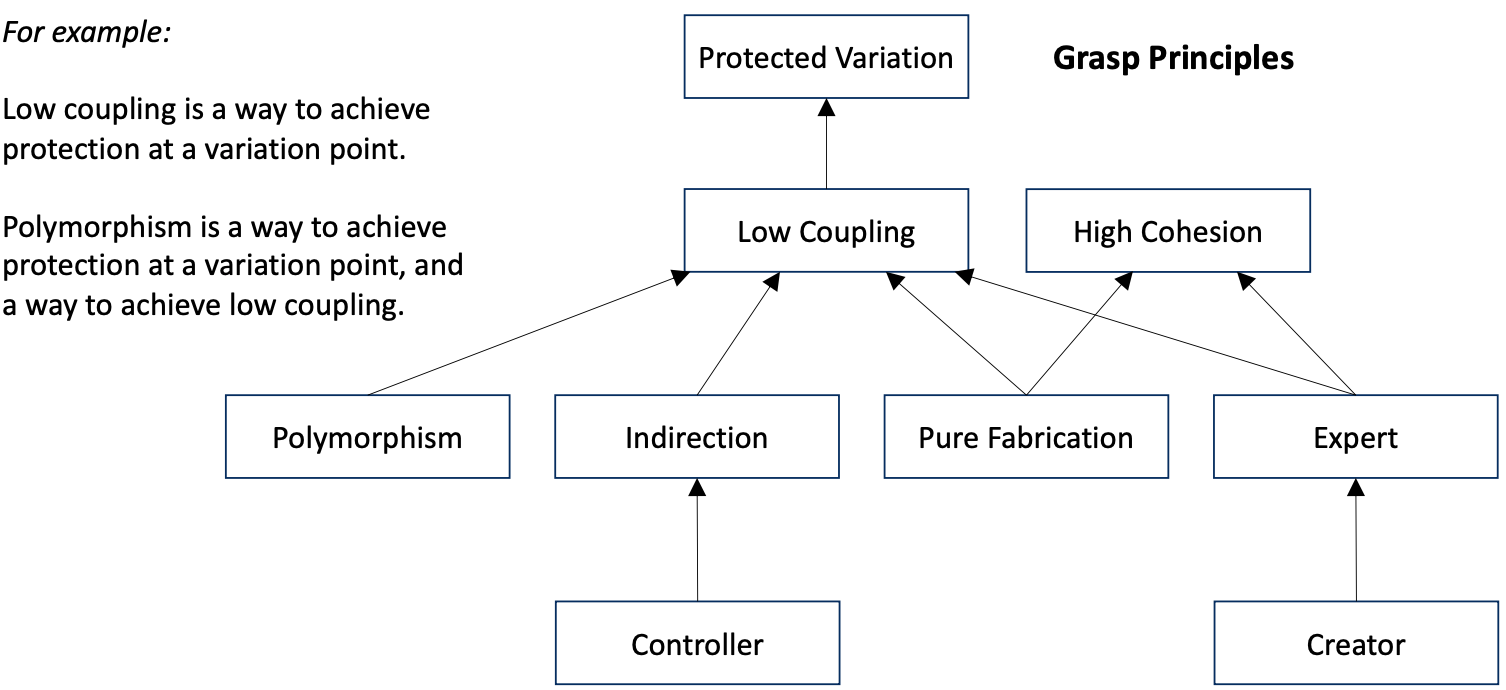
\includegraphics[width=\linewidth]{figs/relationship-of-grasp-principles.png}\\
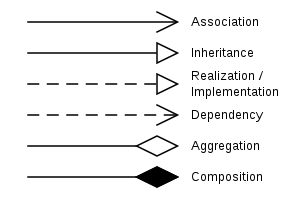
\includegraphics[width=\linewidth]{figs/uml-notation.png}\\
\begin{itemize}
    \item \textbf{Creator:} Who should be responsible for creating a new instance of a class?\\
    \textit{Answer} Assign class B responsibility to create instance of class A if one of these is true:
    \begin{itemize}
        \item B contains or compositely aggregates A
        \item B records A
        \item B closely uses A
        \item B has the initialising data that A needs
    \end{itemize}
    \textit{Contraindications} If creation of objects has significant complexity, e.g., using recycled instances for performance, or conditionally creating an instance from one of a family of similar classes based upon some external property value or other context information, then use a Factory pattern instead.
    \item \textbf{Information expert:} Who has the information necessary to fulfil responsibilities?\\
    \textit{Answer} Assign a responsibility to the class that has the information needed to fulfil it.\\
    \textit{Contraindications} In some situations, a solution suggested by Expert is undesirable because of problems with the resulting dependencies.
    \item \textbf{Low coupling:} How can the coupling between two classes be minimised?\\
    \item \textbf{High cohesion:} How can the responsibilities of a class be appropriately assigned to ensure that the class has high cohesion?\\
    \item \textbf{Controller:} What first object beyond the UI layer receives and coordinates (or controls) a system operation?\\
    \textit{Answer} Use a Controller object to deal with major system events.\\
    \textit{Contraindications} If the system operation is simple, and the system has only one or two layers, then the Controller may be unnecessary.
    \item \textbf{Indirection:} How can indirection be used to increase flexibility and reusability?\\
    \textit{Answer} Assign responsibility to an intermediate object to mediate between other components or services to reduce the coupling between them.\\
    \textit{Contraindications} If the indirection adds complexity with little benefit, then it should be avoided.
    \item \textbf{Pure fabrication:} Where can an additional class be inserted that does not represent a problem domain concept, and that has no superclass?\\
    \textit{Answer} Assign a highly cohesive set of responsibilities to an artificial or convenience class that does not represent a problem domain concept.\\
    \textit{Contraindications} If the class is not cohesive, then it should be avoided.
    \item \textbf{Polymorphism:} How can polymorphism be used to simplify client use of entities and reduce coupling? How can we produce reusable code?\\
    \textit{Answer} When there are related behaviour but only differ by the type, assign responsibility for the behaviour using polymorphic operations. Polymorphism can be achieved by using inheritance or interfaces.\\
    \textit{Contraindications} If the use of polymorphism adds complexity with little benefit, then it should be avoided.
    \item \textbf{Protected variations:} How can we design objects, subsystems, and systems so that the variations in those elements that are likely to change are encapsulated in well-defined, stable areas?\\
    \textit{Answer} Identify points of predicted variation and encapsulate them.\\
    \textit{Contraindications} If the use of protected variations adds complexity with little benefit, then it should be avoided.
\end{itemize}
